\documentclass[12pt, twoside,a4paper]{article}
\oddsidemargin = 10pt
\textwidth = 430pt

\usepackage{fullpage}	 %to make smaller margins
\usepackage{graphicx}
%\usepackage[utf8]{inputenc}
%\usepackage[T1]{fontenc}
%\usepackage{url}

\usepackage[hidelinks]{hyperref}
\usepackage{pdfpages}
\usepackage{placeins}
\usepackage{graphicx}
\usepackage[font=small,labelfont=bf]{caption}
\usepackage{subfig}

%\usepackage{subcaption}
\usepackage{enumerate}
\usepackage{amsmath}
\usepackage{listings} %for showing program code
\usepackage{bm}
\usepackage{wrapfig}
\usepackage{lipsum}
\usepackage{float}
\usepackage{titlesec}	
\usepackage{amsfonts}
\usepackage{amssymb}
\usepackage[comma,authoryear]{natbib}
\usepackage{epstopdf}
\usepackage{array}
\usepackage{blindtext}

%\titlespacing*{\chapter}{0pt}{-10pt}{20pt}
%\titleformat{\chapter}[display]{\normalfont\huge\bfseries}{}{35pt}{}

\setlength{\intextsep}{0pt} %to make wrapfigures beautiful
%\setlength{\oddsidemargin}{0.5cm}
%\setlength{\evensidemargin}{-0.5cm}
\begin{document}
My progress this week:

\section{step1}
It works for one light, positions and normals are rendered correctly into the Gbuffer. WE can see in the second picture that the ear of the bunny correctly takes the same values as \emph{above} the ear.

\vspace{1cm}
\begin{figure}[here]
\centering
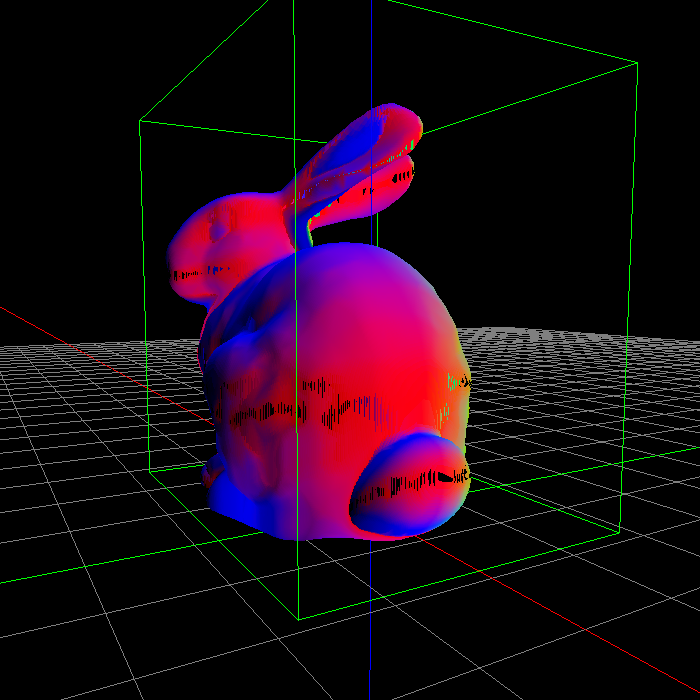
\includegraphics[width=0.8\textwidth]{rendernormals}
\caption{Render of the normals in the bunny.}
\end{figure}

\clearpage
\begin{figure}[here]
\centering
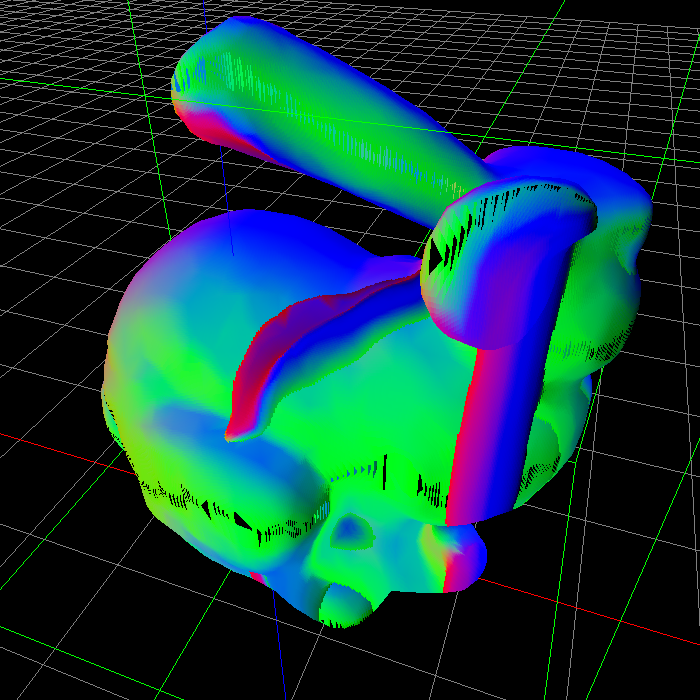
\includegraphics[width=0.8\textwidth]{normals_detail}
\caption{Render of the normals in the bunny - closeup.}
\end{figure}
\clearpage
\section{Step2}
The render to cubemap step is implemented (without sampling and dipoles, it just renders depth and white color for now). 

\vspace{1cm}

\begin{figure}[here]
\centering
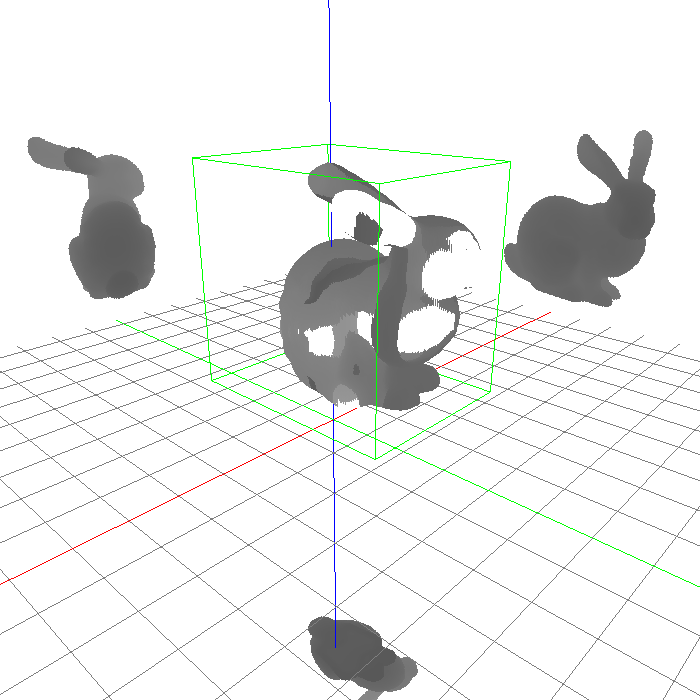
\includegraphics[width=0.8\textwidth]{cubemap}
\caption{Bunny rendered on the cubemap faces.}
\end{figure}

\clearpage
\section{Step3}
Some problems still in the combination of the cubemap from step 2. Seems like there is an offset in the rendering (problem with the view matrices of the previous step probably).

\vspace{1cm}

\begin{figure}[here]
\centering
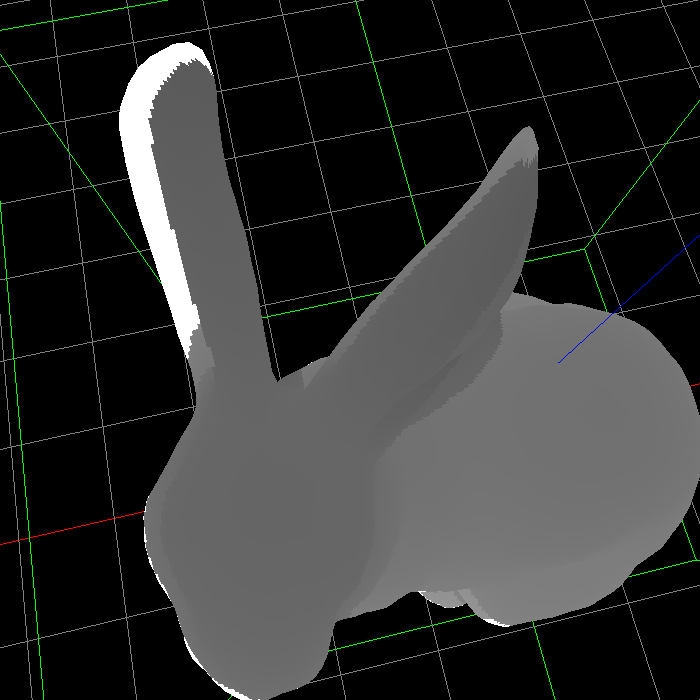
\includegraphics[width=0.8\textwidth]{offset}
\caption{Small offset when trying to map the +Z face on the bunny.}
\end{figure}


\end{document}
